\problemname{Kulramen}

\begin{figure}[h] 
\begin{center}
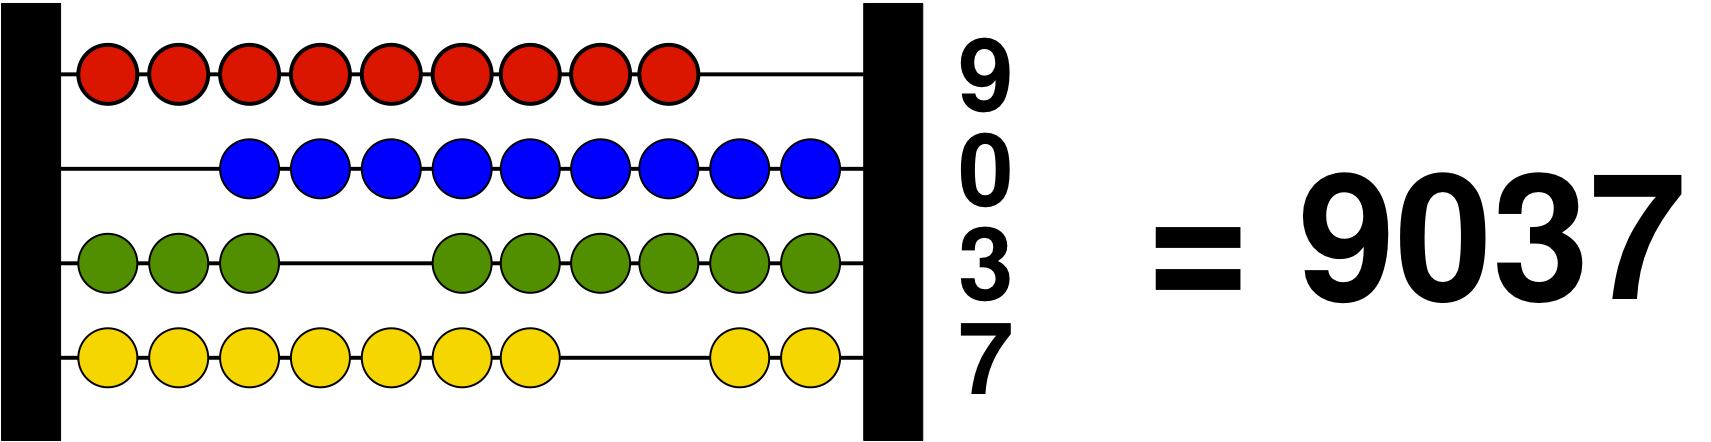
\includegraphics[width=10cm]{kulram0.png}
\caption{Så här kunde Simons kulram (med $R=4$) se ut innan han började äta
  upp kulorna. Då var det lätt att översätta ställningen till ett decimaltal.}
\end{center} 
\end{figure}
\vspace{-2cm}

Lille Simon har fått en kulram i present. Kulramen har $R$ rader och i
varje rad fanns från början 9 kulor, så att man kunde representera
$R$-siffriga decimaltal -- en siffra på varje rad. Om en rad hade $X$
kulor på vänstra sidan, sedan ett mellanrum och övriga kulor på höger sida representerade raden siffran X.

Tyvärr tyckte Simon att kulorna på ramen såg väldigt smaskiga ut, och åt helt enkelt upp några kulor. Det finns dock minst en kula kvar på varje rad.

Simon lärde sig snabbt att räkna på sin nya kulram. Han representerar
talet där alla kulor är på högersidan som talet 0, och adderar sedan 1
precis som han hade gjort på en vanlig kulram, genom att flytta en
kula från höger till vänster på den nedersta raden som har någon kula
kvar på höger sida (låt oss kalla den {\em flyttningsraden}) samt
flytta alla kulor på raderna nedanför flyttningsraden till höger sida
(om inte flyttningsraden är den nedersta raden). Om 1 adderas när alla
kulorna på {\em alla} rader redan är på vänster sida (så att det inte finns någon flyttningsrad) blir resultatet 0.

\begin{figure}[h] 
\begin{center}
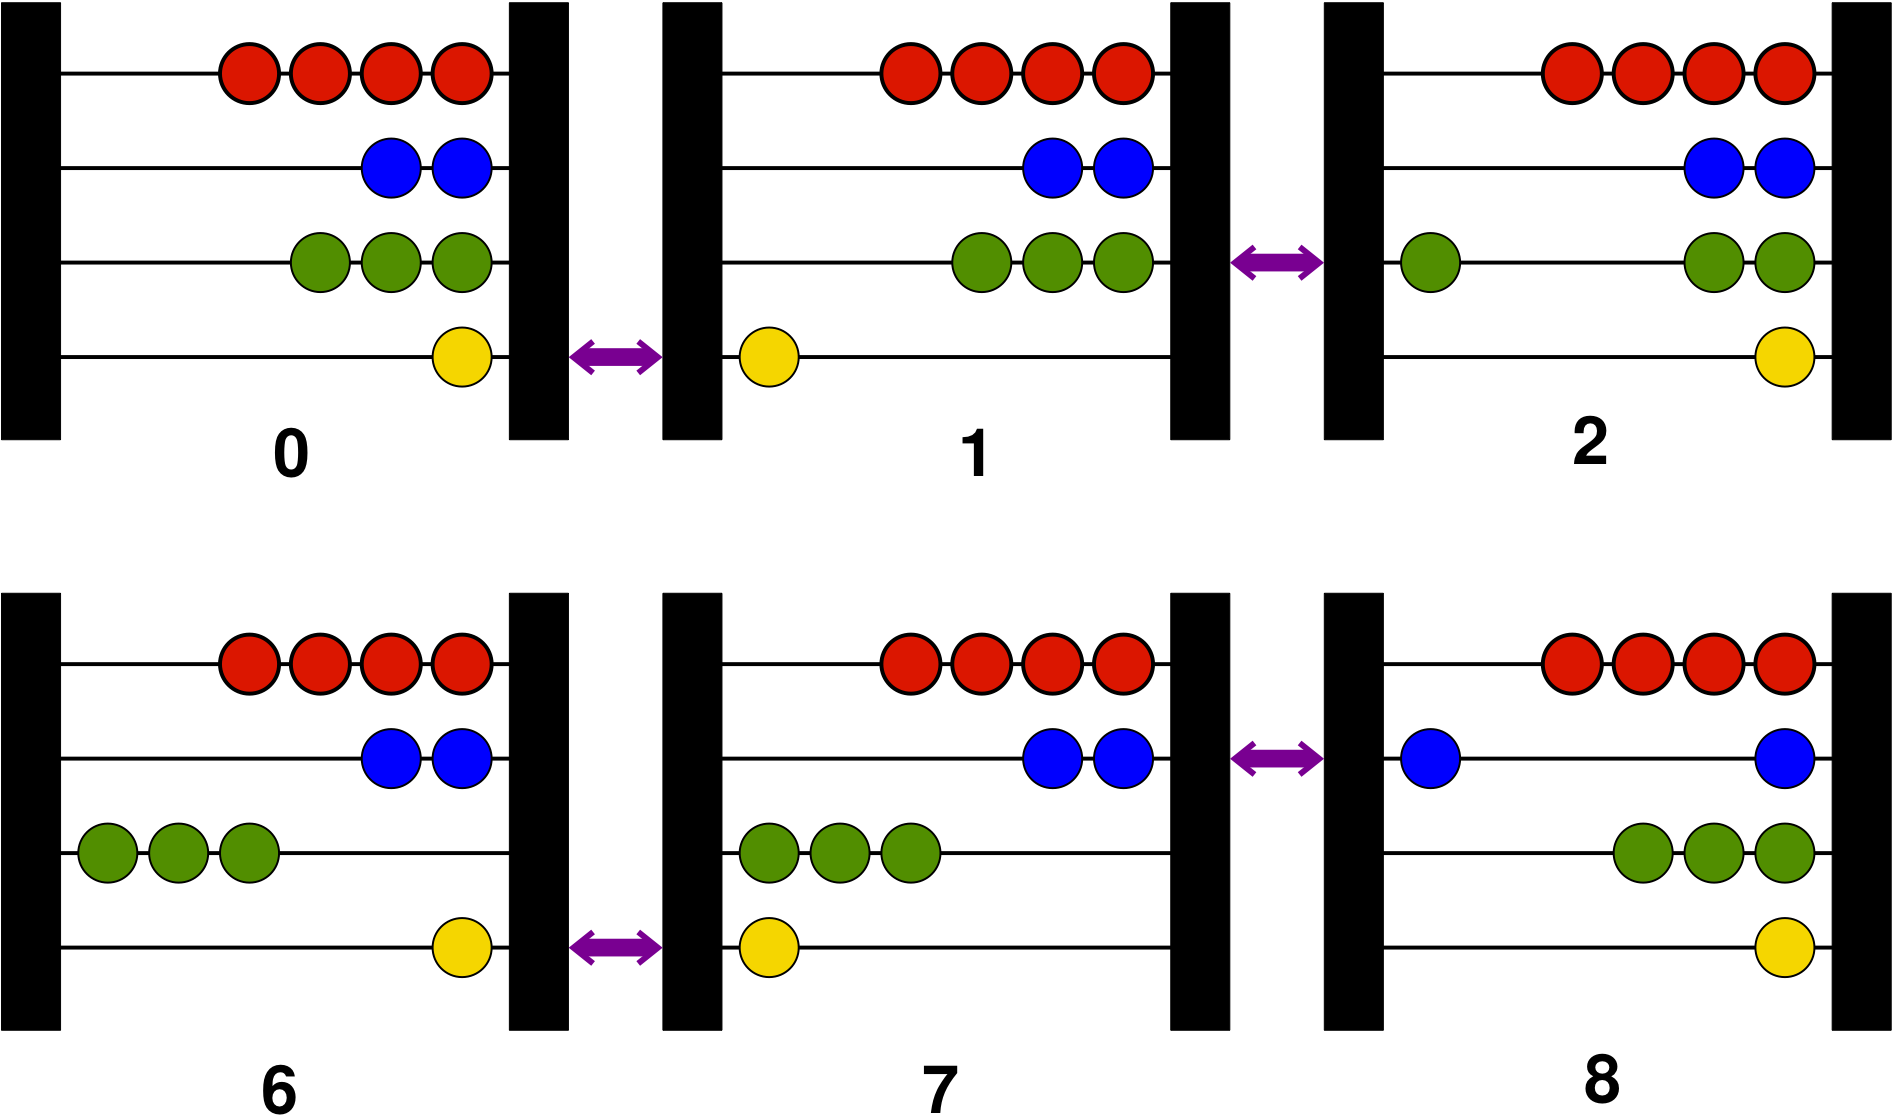
\includegraphics[width=8cm]{kulram.png}
\caption{Några exempel på hur Simon adderar 1 på den kulram som återfinns i de två första exemplen. Dubbelpilen
  markerar ``flyttningsraden'' vid de olika additionerna.}
\end{center} 
\end{figure}

Simon börjar dock tröttna på allt flyttande och skulle behöva hjälp
att skriva ett program som, givet ett visst utgångsläge på kulramen,
räknar ut hur kulramen ser ut när han $N$ gånger har adderat
1.

\section*{Indata}
På första raden står antalet rader $R$. Därefter följer $R$ rader med vardera två heltal, antalet kulor
till vänster respektive höger på varje rad (uppifrån och ned). Slutligen finns en rad med 
det positiva heltalet $N$. 

\section*{Utdata} 

Programmet ska skriva ut $R$ rader med två tal på
varje rad: antalet kulor till vänster respektive höger på varje rad
efter additionerna.

\section*{Poängsättning}

För testfall värt $1$ poäng gäller att $R=4$,  $N\le 100$, och det finns 2 kulor
på varje rad.\\
För testfall värda ytterligare $2$ poäng gäller att $R=4$ och $N\le 10,000$.\\
För testfall värda $2$ poäng gäller att $R\le 9$ och $N\le 1,000,000,000$.

